% soctepmlate unofficial - SOČ = Středoškolská odborná činnost - Czech competition
% Author: Vojtěch Boček
% Edit by: Jaroslav Páral
% Version: 2018-02-12
% Source code: https://github.com/RoboticsBrno/soctemplate/
% Base on: http://www.jcmm.cz/cz/sablona-soc.html
% License: CC BY 4.0

\documentclass{template/socthesis}

\usepackage{subcaption}
\usepackage{amsmath}
\usepackage{enumitem}
\usepackage{siunitx}
\usepackage{listings}
\usepackage{float}
\usepackage{caption}
\usepackage{glossaries}
\usepackage{titlesec}
\usepackage[T1]{fontenc}

\addbibresource{text.bib}

\titleformat{\chapter}[display]{\normalfont\huge\bfseries}{\chaptertitlename\ \thechapter}{20pt}{\Huge}
% \titlespacing*{⟨command ⟩}{⟨left ⟩}{⟨before-sep ⟩}{⟨after-sep ⟩}[⟨right-sep ⟩]
\titlespacing*{\chapter}{0pt}{5pt}{20pt}

\titlecz{Webový portál BurzaŠkol.Online}
\titleen{BurzaŠkol.Online Web Portal}
\author{Vít Falta}
\field{18}
\school{DELTA - Střední škola informatiky a ekonomie, s.r.o.}
\mentor{RNDr. Jan Koupil, Ph.D.}
\mentora{RNDr. Jana Koupila, Ph.D.}

% Změňte, pokud se liší
\region{Pardubický}
\placefooter{Pardubice 2021}


\newcommand{\bso}{\textit{BurzaŠkol.Online}}
\newcommand{\expl}[2]{#1 -- #2}
\newcommand{\emptyLine}{\vspace{\baselineskip}}
\newcommand{\inlaravel}{ve \gls{framework}u \nameref{subsub:laravel}}

\newcommand{\important}[1]{\begin{center}#1\end{center}}
\newcommand{\subsubsubsection}[1]{\emptyLine{\setlength{\parindent}{0cm}\textbf{#1}}}

\makeglossaries

\newacronym{ssh}{SSH}{Secure Shell}
\newacronym{dos}{DoS}{Denial of Service}
\newacronym{ddos}{DDoS}{Distributed Denial of Service}
\newacronym{fd}{FD}{File Descriptor}
\newacronym{ip}{IP}{Internet Protocol}

\newacronym{hw}{HW}{Hardware}
\newacronym{sw}{SW}{Software}

\newacronym{dns}{DNS}{Domain Name System}
\newacronym{ntp}{NTP}{Network Time Protocol}

\newacronym{udp}{UDP}{User Datagram Protocol}

\newacronym{sql}{SQL}{Structured Query Language}

\newacronym{webserver}{webserver}{Webový server}
\newacronym{http}{HTTP}{Hyper Text Transport Protocol}
\newacronym{html}{HTML}{Hyper Text Markup Language}
\newacronym{css}{CSS}{Cascading Stylesheets}
\newacronym{js}{JS}{JavaScript}
\newacronym{ws}{WS}{Web Sockets}
\newacronym{ssl}{SSL}{Secure Sockets Layer}
\newacronym{wysiwyg}{WYSIWYG}{What You See Is What You Get}

\newacronym{stdout}{STDOUT}{Standard Output}
\newacronym{stdin}{STDIN}{Standard Input}
\newacronym{stderr}{STDERR}{Standard Error}

\newacronym{php}{PHP}{Rekurzivní název programovacího jazyka PHP: Hypertext Preprocessor}

\newacronym{ide}{IDE}{Integrovaná vývojová prostředí}

\newacronym{gui}{GUI}{Grafické uživatelské rozhraní}

\newacronym{http-sse}{SSE}{Server-sent events}

\newacronym{msmt}{MŠMT}{Ministerstvo školství, mládeže a tělovýchovy České republiky}

\newacronym{aws}{AWS}{Amazon Web Services}
\newacronym{aws-ses}{SES}{Simple Email Service}

\newacronym{dmz}{DMZ}{Demilitarized zone}

\newacronym{smtp}{SMTP}{Simple Mail Transfer Protocol}
\newacronym{imap}{IMAP}{Internet Message Access Protocol}
\newacronym{wss}{WSS}{WebSocket Secure}

\newacronym{csrf}{CSRF}{Cross-site request forgery}
\newacronym{xss}{XSS}{Cross-site scripting}

\newglossaryentry{ci-cd}
{
    name={CI/CD},
    description={Continuous integration and continuous delivery. Mechanismus pro automatické testování a nasazování softwaru}
}

\newglossaryentry{dkim}
{
    name={DKIM},
    description={DomainKeys Identified Mail. Systém certifikátů pro ověření autenticity odesílatele emailu}
}

\newglossaryentry{scaffolding}
{
    name={scaffolding},
    description={Předpřipravená souborová struktura pro vývoj projektu}
}

\newglossaryentry{perl}
{
    name={Perl},
    description={Rodina dvou vyšších dynamických programovacích jazyků Perl 5 a Perl 6}
}

\newglossaryentry{cgi}
{
    name={CGI},
    description={Common Gateway Interface. Rozhraní umožňující webovým serverům spouštět terminálové aplikace}
}

\newglossaryentry{debugger}
{
    name={Debugger},
    plural={debuggery},
    description={Programy určené pro ladění programů}
}

\newglossaryentry{round-robin}
{
    name={Round Robin},
    description={Algoritmus sekvenčně rotující backendové servery ze skupiny dostupných serveru, tj. jeden po druhém}
}
\newglossaryentry{least-con}
{
    name={Least Connections},
    description={Algoritmus vybírající server podle nejnižšího počtu právě zpracovávaných požadavků}
}
\newglossaryentry{ip-hash}
{
    name={IP Hash},
    description={Algoritmus využívající klientskou IP adresu pro vybrání backendového serveru}
}
\newglossaryentry{on-demand}
{
    name={on-demand},
    description={Ve chvili potřeby. Typ škálování, při kterém se daný zdroj automaticky přizpůsobuje objemu uživatelských požadavků}
}

\newglossaryentry{real-time}
{
    name={real-time},
    description={V reálném čase. Zobrazování, či provádění akcí, v současnou chvíli nebo s minimální odezvou}
}

\newglossaryentry{open-source}
{
    name={open-source},
    description={Software s otevřeným zdrojovým kódem}
}

\newglossaryentry{mvp}
{
    name={MVP},
    description={Minimum Viable Product. Nejmenší možná verze produktu, která je schopná plnit zadaný účel}
}

\newglossaryentry{pubsub}
{
    name={pub-sub},
    description={Publish-subscribe. Způsob předávání zpráv. Zprávy jsou organizovány do kanálů. Klienti se do těchto kanálů mohou zapojit a dostávat příslušné zprávy}
}

\newglossaryentry{framework}
{
    name={framework},
    description={Předpřipravený základ pro tvorbu aplikací},
    plural={frameworky}
}

\newglossaryentry{orm}
{
    name={ORM},
    description={Object-Relational Mapper. Software sloužící pro konverzi dat mezi relačním a objektovým modelem},
}
\newglossaryentry{php-router}
{
    name={směrovač},
    description={Software rozhodující o tom, jaký kód bude spuštěn v odpovědi na uživatelský požadavek},
}
\newglossaryentry{php-templater}
{
    name={šablonovací knihovna},
    description={Knihovna ulehčující generování HTML},
}
\newglossaryentry{bug}
{
    name={Bug},
    description={Chyby programu zapříčiněné chybou, či nepozorností programátora},
    plural={bugy}
}
\newglossaryentry{http-polling}
{
    name={HTTP Polling},
    description={Periodické stahování dat za pomoci separátních HTTP požadavků.},
    plural={bugy}
}



%%% TODO: What to use?
\newacronym{rdbms}{RDBMS}{Relational Database Management System}
%%%\newacronym{rdbms}{SŘRBD}{Systém řízení relační báze dat}

\newglossaryentry{dql}
{
    name={DQL},
    description={Jazyk sloužící pro vytváření dotazů nad daty. DQL je někdy zmiňováno jako součást \gls{dml}},
    first={Data Query Language (DQL)}
}
\newglossaryentry{dml}
{
    name={DML},
    description={Jazyk sloužící pro manipulaci, vytváření a mazání dat},
    first={Data Manipulation Language (DML)}
}
\newglossaryentry{dcl}
{
    name={DCL},
    description={Jazyk sloužící pro řízení přístupu k datům},
    first={Data Control Language (DCL)}
}
\newglossaryentry{ddl}
{
    name={DDL},
    description={Jazyk sloužící pro definování struktury dat a ostatních databázových objektů},
    first={Data Definition Language (DDL)}
}
\newglossaryentry{tcl}
{
    name={TCL},
    description={Jazyk sloužící pro vytváření a správu transakcí},
    first={Transaction Control Language (TCL)}
}

\newacronym{acid}{ACID}{Atomicity, consistency, isolation, durability}

\newglossaryentry{sql-trigger}
{
    name={Trigger},
    plural={triggery},
    description={\acrshort{sql} kód spuštěný v návaznosti ná různé události}
}
\newglossaryentry{sql-saved-procedure}
{
    name={Uložená procedura},
    plural={uložené procedury},
    description={Pojmenovaný \acrshort{sql} kód uložený v \acrshort{rdbms}, který můžeme opakovaně spouštět}
}

\begin{document}
\sloppy

	\maketitle
	
	\makecopyrightstatement{V~Pardubichích}
	
	\makethanks{Děkuji svému školiteli RNDr. Janu Koupilovi, Ph.D. za obětavou pomoc, podnětné připomínky a nekonečnou trpělivost, kterou mi během práce poskytoval. \
  Dále bych chtěl poděkovat panu Jiřímu Formánkovi za poskytnutí myšlenky projektu, podnětů a propagace projektu.\
  \par \
  Na závěr bych chtěl poděkovat pánům Matěji Půhonému a akademickému malíři~Danielu~Václavíkovi za grafický návrh a pomoc s grafickou stránkou projektu.}
	
	\pagestyle{empty}
	
	\section*{Anotace}
	Cílem této práce je vytvořit online platformu, která umožní nahrazení klasických burz škol v~České Republice, pomocí moderních webových technologií v~době pandemie Covidu-19. Tato platforma zprostředkuje kontakt mezi středními školami a žáky 9. ročníků základních škol v~době, kdy jsou klasické burzy škol z~hygienických důvodů nemožné.
	
	\subsection*{Klíčová slova}
	burza škol; webová stránka; www; online; online platforma
	
	\vspace{20mm}
	
	\section*{Annotation}
	The goal of this work is to create an online platform that will allow the replacement of traditional school presentation fairs in the Czech Republic using modern web technologies during the Covid-19 pandemic. This platform mediates contact between secondary schools and pupils in the 9th grade of primary schools at a time when traditional school exchanges are impossible due to hygienic restrictions.

	\subsection*{Keywords}
	school exchange; web page; www; online; online platform
	
	\newpage
	\pagestyle{plain}
	
  \tableofcontents % vysází obsah
	
	%%% Začátek práce
	\setcounter{figure}{0}
	\setcounter{table}{0}
	\newpage
	
	
	%%% Úvod
	\chapter*{Úvod}
\addcontentsline{toc}{chapter}{Úvod} % přidá položku úvod do obsahu

Každý podzim se v~České Republice konají tzv. Výstavy středních škol, nebo také Burzy, či Veletrhy vzdělávání (názvy se liší kraj od kraje). Hromadné akce na kterých se střední školy snaží zaujmout co nejvíce žáků \expl{9. tříd základních škol}{deváťáků} a vylíčit svou školu v~nejlepším světle.

Deváťáci mají možnost si v~jeden čas a na jednom místě prohlédnout nabídky jednotlivých škol. Pokud je nějaká škola zaujme mají možnost získat podrobnější informace od zástupců dané školy. 

Vzhledem k~pandemické situaci roku 2020 spojené s~nemocí COVID-19, ale nebylo možné tyto Burzy uspořádat. Systém \bso{} umožnil přesunutí celého náboru deváťáků do virtuálního prostředí internetu.

\section*{Jak to funguje?}
\bso{} je internetový portál zprostředkující kontakt mezi deváťáky a středními školami za pomoci on-line video konferencí (nejčastěji MS~Teams\cite{ms-teams}, Google~Meet\cite{google-meet}, Zoom\cite{zoom}, \cdots). Běžnému návštěvníkovi portál nabízí seznam virtuálních burz škol, ve kterém má každá burza přiřazený termín a lokalitu konání.

Střední školy se mohou registrovat k~jednotlivým burzám a vložit odkaz na svou on-line konferenci. V~den konání burzy se mohou deváťáci kliknutím na odkaz připojit do on-line konference vybrané školy.

Střední školy mají na portále založený svůj profil s~informacemi o~škole, seznam oborů a další informace jako informační brožura, či výsledky v~soutěžích.

Odkaz na repositář s~kódem: \href{https://github.com/GrimirCZ/delta-burza}{https://github.com/GrimirCZ/delta-burza}.

\pagebreak

%Účelem je stručně a věcně seznámit se záměrem a řešením tématu, důvodem jeho volby, stručně nastínit problém, který má být řešen (a proč); cíl práce (co je předmětem řešení, jakým způsobem se postupuje a k~čemu se má dospět -- co bude výsledkem; cíl práce je 

	
	\chapter{Teoretická část}
	\label{chap:teoretical-part}
	
	%%% Fungování burz škol
	\section{Serverová infrastruktura}\label{sub:server-architecture}

Tato sekce popisuje prvky serverové infrastruktury, které jsou nasazeny v~reálném řešení \bso{}.

\subsection{Load Balancery}\label{sub:load-balancing}

Load balancer\cite{load-balancer} je prvek serverové infrastruktury určený k~rozložení příchozích požadavků na skupinu backendových serverů. K~rozložení požadavků je využíváno nejrůznějších algoritmů, jako například \gls{round-robin}, \gls{least-con}, či \gls{ip-hash}. Dělíme je na \acrshort{sw} load balancery a \acrshort{hw} load balancery. 

\acrshort{hw} load balancery jsou zpravidla proprietární a nákladná řešení. Vysokého výkonu dosahují využitím dedikovaných \acrshort{hw} akcelerátorů. Jediné způsoby jejich škálování jsou zakoupení více fyzických strojů, či zakoupení silnějších strojů.

\acrshort{sw} load balancery jsou distribuovány ve formě uživatelských aplikací spustitelných na běžném hardwaru, či ve virtuálních strojích cloudových providerů. Škálovatelnost je tedy velice triviální. V~porovnání s~\acrshort{hw} load balancery stačí pouze \gls{on-demand} zakoupit virtuální stroj s~odpovídajícím výpočetním výkonem.  Tato vlastnost činí z~\acrshort{sw} load balancerů velice flexibilní řešení, ideální pro agilní cloudové prostředí.

\subsection{Objektová úložiště}


Objektové úložiště je typ úložiště určený k~ukládaní nestrukturovaných dat. Na rozdíl od tradičních způsobů ukládání dat, jakými jsou souborové systémy a bloková úložiště, pracují objektová úložiště\cite{object-storage} s~daty jako se samostatnými objekty. Každý objekt obsahuje data samotná, uložená v~jejich nativním formátu, a metadata. Metadata obsahují informace jako přístupová práva objektu, unikátní globální identifikátor a další přidružené informace, například formát uložených dat. Díky adresaci za pomocí globálních identifikátorů je možné objekty transparentně přesouvat. Tato vlastnost nám poskytuje nezávislost dat na použitém záznamovém médiu.

Je tedy například možné přesunout málo používané objekty z~diskového úložiště na úložiště založené na magnetické pásce. Na druhou stranu ale také můžeme transparentně přesunout často požadované objekty z~úložiště do pracovní paměti pro rychlý přístup.

Objektová úložiště dovolují ukládání velkého objemu nestrukturovaných dat. Je proto ideální jako úložiště pro uživatelské obrázky, dokumenty a zálohy. Díky své flexibilitě jsou objektová úložiště výrazně levnější než například bloková úložiště.

\subsection{Relační databáze}

Relační databáze\cite{relational-database} jsou úložiště strukturovaných dat, založená na tzv.\ relačním modelu. Relační model organizuje data do \emph{tabulek}, \expl{\emph{řádků}}{záznamů} a \emph{sloupců}. Vzájemné vztahy mezi záznamy jsou reprezentovány \expl{\emph{relacemi}}{shodnými hodnotami dvou sloupců}. 

Software implementující relační databáze se nazývá \acrfull{rdbms}. \acrshort{rdbms} dále obsahuje implementaci některého z~dotazovacích jazyků, např. \acrshort{sql}, a podporu funkcí jako jsou \acrshort{acid}, \glspl{sql-trigger} a \glspl{sql-saved-procedure}.

\subsubsection{SQL}

Pro dotazování a správu dat uchovaných v~\acrshort{rdbms} se využívá standardizovaný jazyk \acrshort{sql} (\acrlong{sql})\cite{sql}. Díky němu můžeme data analyzovat a získávat z~nich informace. Data můžeme shlukovat, transformovat a zkoumat pomocí nejrůznějších statistických funkcí.

\subsubsection{Spravované databáz}\label{subsub:managed-databases}

Provize a správa databází je velice komplikovaná. Je třeba řešit replikaci, a také automatické škálování. Spravované databáze\cite{managed-databases} se snaží tyto problémy řešit poskytováním předpřipravených databázových instancí, u~kterých je automaticky řešena provize a škálování. Většina spravovaných databází dále poskytuje velice bezpečné nastavení vyladěné pro maximální bezpečnost a výkon databáze. To nám dovoluje se starat pouze o~databázové objekty a uživatelské účty, tedy aspekty které přímo ovlivňují naši aplikaci.

Další výhodou spravovaných databází je poskytování různých metrik a varování, která nám ukazují detailnější informace o~stavu a provozu databáze. Spravovaná databáze je například schopná detekovat tabulky bez primárního klíče a zaslat upozornění databázovému administrátorovi, či zobrazovat detailní \gls{real-time} statistiky o~propustnosti databáze.

\subsection{Webové servery}

\acrfull{webserver}\cite{webserver} je klíčový prvek infrastruktury webové aplikace. Hlavní rolí \acrshort{webserver}u, jak už název napovídá, je poskytování webových stránek. Moderní \acrshort{webserver}y podporují širokou škálu protokolů jako je \acrfull{http}, \acrfull{ws}, či \acrfull{ssl}. Pro standardní internetovou komunikaci využívají \acrshort{webserver}y síťové porty 80 pro nešifrovanou komunikaci a 443 pro šifrovanou komunikaci. 

Většina \acrshort{webserver}ů poskytuje obsah dvěma způsoby, staticky a dynamicky. Statický obsah je poskytován ze souborů uložených na \acrshort{webserver}u samotném. Dynamický obsah je na druhou stranu generován samostatným aplikačním serverem, který poté využívá \acrshort{webserver} jako komunikační bránu. Některé \acrshort{webserver}y mají schopnost přímo provádět aplikační kód a separátní server není potřeba. Pro vytváření dynamických stránek můžeme například využít \acrshort{php}, \Gls{perl}, či různé \Gls{cgi} skripty. Statický obsah je ideální pro poskytování obsahu jako jsou obrázky, či klientské skripty. Dynamický obsah se na druhou stranu využívá pro obsluhu formulářů, či generování sestav.

	
	\section{Aplikační architektura}
\label{sub:app-architecture}

Tato sekce popisuje technologie využité při vývoji aplikace \bso{}.

\subsection{HTTP}

\acrshort{http}\cite{http} je jeden z~klíčových internetových protokolů. Mezi jeho hlavní přednosti patří jeho textová podoba a bezstavovost. Po síti tedy cestují pouze jednoduše stravitelné textové řetězce, převážně čitelné i pro člověka. Díky tomu je oproti ostatním přenosovým protokolům jednoduše použitelný a implementovatelný. Bezstavovost znamená, že jednotlivé \acrshort{http} požadavky na sebe nijak nenavazují a jsou plně nezávislé.

\subsection{PHP}
\label{sub:php}

\acrshort{php}\cite{php} je skriptovací jazyk vytvořený v~roce 1994 pro snadný vývoj dynamických a interaktivních webových aplikací. Hlavními přednostmi jazyka \acrshort{php} je dynamický typový systém, extenzívní standardní knihovna a hluboká integrace s~klíčovými webovými technologiemi. Funkcionalita jazyka PHP je dále rozšiřována velkým množstvím knihoven a frameworků. Pro jednoduchou správu těchto knihoven je využíván správce balíčků Composer\cite{composer}.

\subsection{PHP Frameworky}

Vytváření rozsáhlé a propracované webové aplikace je těžký a dlouho trvající úkol. Z~tohoto důvodu se využívají tzv. \emph{\glspl{framework}}. Tyto \glspl{framework} obsahují široké množství nástrojů pro usnadnění vývoje webových aplikací. Mezi nejčastěji poskytované nástroje patří \Gls{orm}\cite{orm}, \gls{php-router}\cite{php-router}, či \gls{php-templater}\cite{php-templater}. Dále může obsahovat nástroje na správu uživatelských sezení a různé další utility. Časté jsou i různé terminálové programy určené k~ulehčení práce s~daným \gls{framework}em, např. pro generování kontrolerů, databázových migrací a správu mezipaměti.

Využitím \gls{framework}u můžeme významně zkrátit čas vývoje aplikace, jelikož autoři \gls{framework}u za nás učinil většinu architekturálních rozhodnutí a implementovali obslužný kód. Nám tedy zbývá pouze byznysová logika naší aplikace a nemusíme řešit věci jako je ukládání často využívaných dat do mezipaměti, či ověřování uživatelů.

Na druhou stranu využití \gls{framework}u sebou nese i jisté nebezpečí. \Gls{framework}y se mezi sebou liší, tudíž zkušenosti s~jedním \gls{framework}em nemusí být přenositelné na druhý. Často je tomu naopak - při používání \gls{framework}u nevhodným způsobem mohou vzniknout velké problémy, především po stránce výkonu aplikace. Dalším velkým nebezpečím mohou být \glspl{bug} samotného \gls{framework}u, jejichž opravou, či obcházením ztrácíme čas určený pro vývoj aplikace samotné.

\subsubsection{Laravel}
\label{subsub:laravel}

Laravel\cite{laravel} je \acrshort{php} \gls{framework} pro snadné tvoření komplexních webových aplikací. Hlavními výhodami \gls{framework}u Laravel je propracovaná, detailní dokumentace a obrovský ekosystém podpůrných knihoven, projektů a služeb, jako např. Laravel Vapor\cite{laravel-vapor} nebo Laravel Nova\cite{laravel-nova}.

\subsection{Webové sokety}

Většina webových aplikací vyžaduje dříve či později nějakou \gls{real-time} funkcionalitu. Je mnoho způsobů, jak tuto funkcionalitu implementovat. Můžeme využít \Gls{http-polling}\cite{http-polling} nebo \Gls{http-sse}\cite{http-sse}. Velká slabina obou těchto přístupů je, že i když máme stále aktuální data ze serveru, tak~neexistuje způsob, jak tyto metody využít pro odesílání požadavků na server. Je proto nutné udělat separátní \acrshort{http} požadavek, což je velice neefektivní.

Protokol \acrfull{ws}\cite{ws} se tento problém snaží řešit poskytováním plně duplexní komunikace mezi klientským programem a serverem. Jelikož se jedná o~protokol cílený na použití ve webových prohlížečích, staví tento protokol nad protokolem \acrshort{http}, který používá pro \expl{navázání komunikace}{handshaking}. Využívá i stejné porty jako protokol \acrshort{http}, port 80 pro nešifrovanou a port 443 pro šifrovanou komunikaci.

\subsubsection{Pusher}
\label{subsub:pusher}

Pusher\cite{pusher} je software stavějící nad \acrshort{ws} protokolem poskytující \gls{pubsub} komunikaci v~reálném čase mezi serverem a klientskými zařízeními. Je vhodný pro aplikace, které nemohou tyto funkcionality poskytovat samy o~sobě, např. stránky napsané v~\acrshort{php}. Pro tyto aplikace poskytuje Pusher jednoduché \acrshort{http} rozhraní, skrze které je možné zprávy zasílat a docílit tím komunikace v~reálném čase.

\subsection{Datový model}

Datový model\cite{data-model} určuje způsob průtok dat, interakcí mezi daty a uložení dat aplikace. Od datového modelu se odvíjí většina aspektů aplikace, např.~způsob fungování nebo rozložení formulářů a přehledů.

Návrh datového modelu je jedna z~nejdůležitějších částí vývoje webové aplikace.  Pokud pří návrhu uděláme chybu můžeme si vývoj aplikace velice ztížit. Na druhou stranu dobře připravený datový model velice zjednodušuje vývoj aplikace, jelikož může sloužit jako referenční manuál pro její rozložení.


	\section{Vývojové prostředí}
\label{sub:development-enviroment}

Pro vývoj softwaru je zapotřebí specializovaných vývojových prostředí. Vývojová prostředí obsahují interpreter, či kompilátor (dle typu jazyka)\cite{interpreter-vs-compiler}, textový editor a další pomocný software, např. linter\cite{linter} nebo jazykový server\cite{language-server}. Hlavním účelem vývojových prostředí je umožnit vývoj softwaru a co nejvíce ho zjednodušit. 

Jelikož je příprava vývojových prostředí náročný a zdlouhavý proces, najdeme řadu postupů, jak jej zjednodušit. Existují různé programy, které vývojové prostředí vytvoří a nastaví a snaží se při tom brát v~potaz nejběžnější nastavení, která by běžný uživatel mohl potřebovat. Jedná se o~programy jako \emph{create-react-app}\cite{create-react-app} a \emph{Artisan Console}\cite{laravel-artisan}. Tyto programy nabízejí funkcionality jako zakládání nového projektu, generování šablon pro různé kusy kódu a spouštění projektu.

Hlavní slabinou těchto programů je, že i když pomáhají s~přípravou projektu, často nepomáhají se samotným vývojem. Tento problém se snaží řešit tzv. \acrfull{ide}\cite{ide}.  

\subsection{Integrovaná vývojová prostředí (IDE)}

Hlavním cílem \acrshort{ide} je pokrýt kompletní vývojový cyklus aplikace. Od založení projektu, přes psaní, až po její vydání. \acrshort{ide} proto obsahuje široké množství nástrojů. Na rozdíl od pomocných programů se ale jedná o~ucelený balíček. Dále často obsahují editor kódu s~inteligentním napovídáním a zvýrazňováním, jednu z~hlavních výhod použití \acrshort{ide}. Samozřejmostí jsou také pokročilé možnosti ladění kódu s~\acrshort{gui} \glspl{debugger} nebo navigování pomocí symbolů.

Pokud by nám základní funkcionalita \acrshort{ide} nestačila můžeme využít dalších zásuvných modulů. Ty jsou poskytovány buďto autorem samotného \acrshort{ide} nebo třetí stranou. Zásuvné moduly poskytují funkcionality jako podporu dalších jazyků, či formátů souborů, rozšíření možností editování textu nebo integraci s~dalšími službami.
	
	\chapter{Realizace projektu}
	\label{chap:practical-part}
	
	\section{Návrh datového modelu}
\label{sub:data-model}

První krok\cite{data-model} při návrhu datového modelu je vypracování zadání a přesné vymezení datových entit, zatím určujeme pouze název a účel entity. Následně musíme definovat relace mezi daty, tedy popsat, jakým způsobem mezi sebou data interagují.

Druhým krokem je vytyčení atributů datových entit. U atributu je třeba určit název, typ dat, která v něm budou uložena, např. datum. Je také nutné určit zda bude atribut držet unikátní hodnoty, např. emailové adresy a zda je atribut povinný nebo zda může nést prázdnou hodnotu, tzv. \emph{null}\cite{null}.

Dalším krokem je adaptace tohoto obecného datového modelu, do modelu specifického pro prostředí, v kterém budou data uložena, např. relační databáze. V tomto kroku dojde k materializaci relací mezi entitami na cizí klíče a intermediate tabulky\cite{intermediate-table}. Podle atributů vytvořených v druhém kroku vytvoříme příslušné sloupce s odpovídajícími datovými typy a omezeními. 

Posledním krokem, který nemusí nutně probíhat v době návrhu, ale může být proveden dodatečně, je vytipování často využívaných dat a vytvoření tzv. \emph{indexů}\cite{index}. Ty slouží pro optimalizaci databázových dotazů a urychlení vyhledávání dat. Tento krok je dobré provést až po vytyčení hlavních dotazů a identifikaci míst, která by indexováním mohla benefitovat. \emph{Přílišné indexování může vést k nárůstu velikosti databáze a zpomalení dotazů!}\cite{bad-indexing}

\begin{figure}[h]
\centering
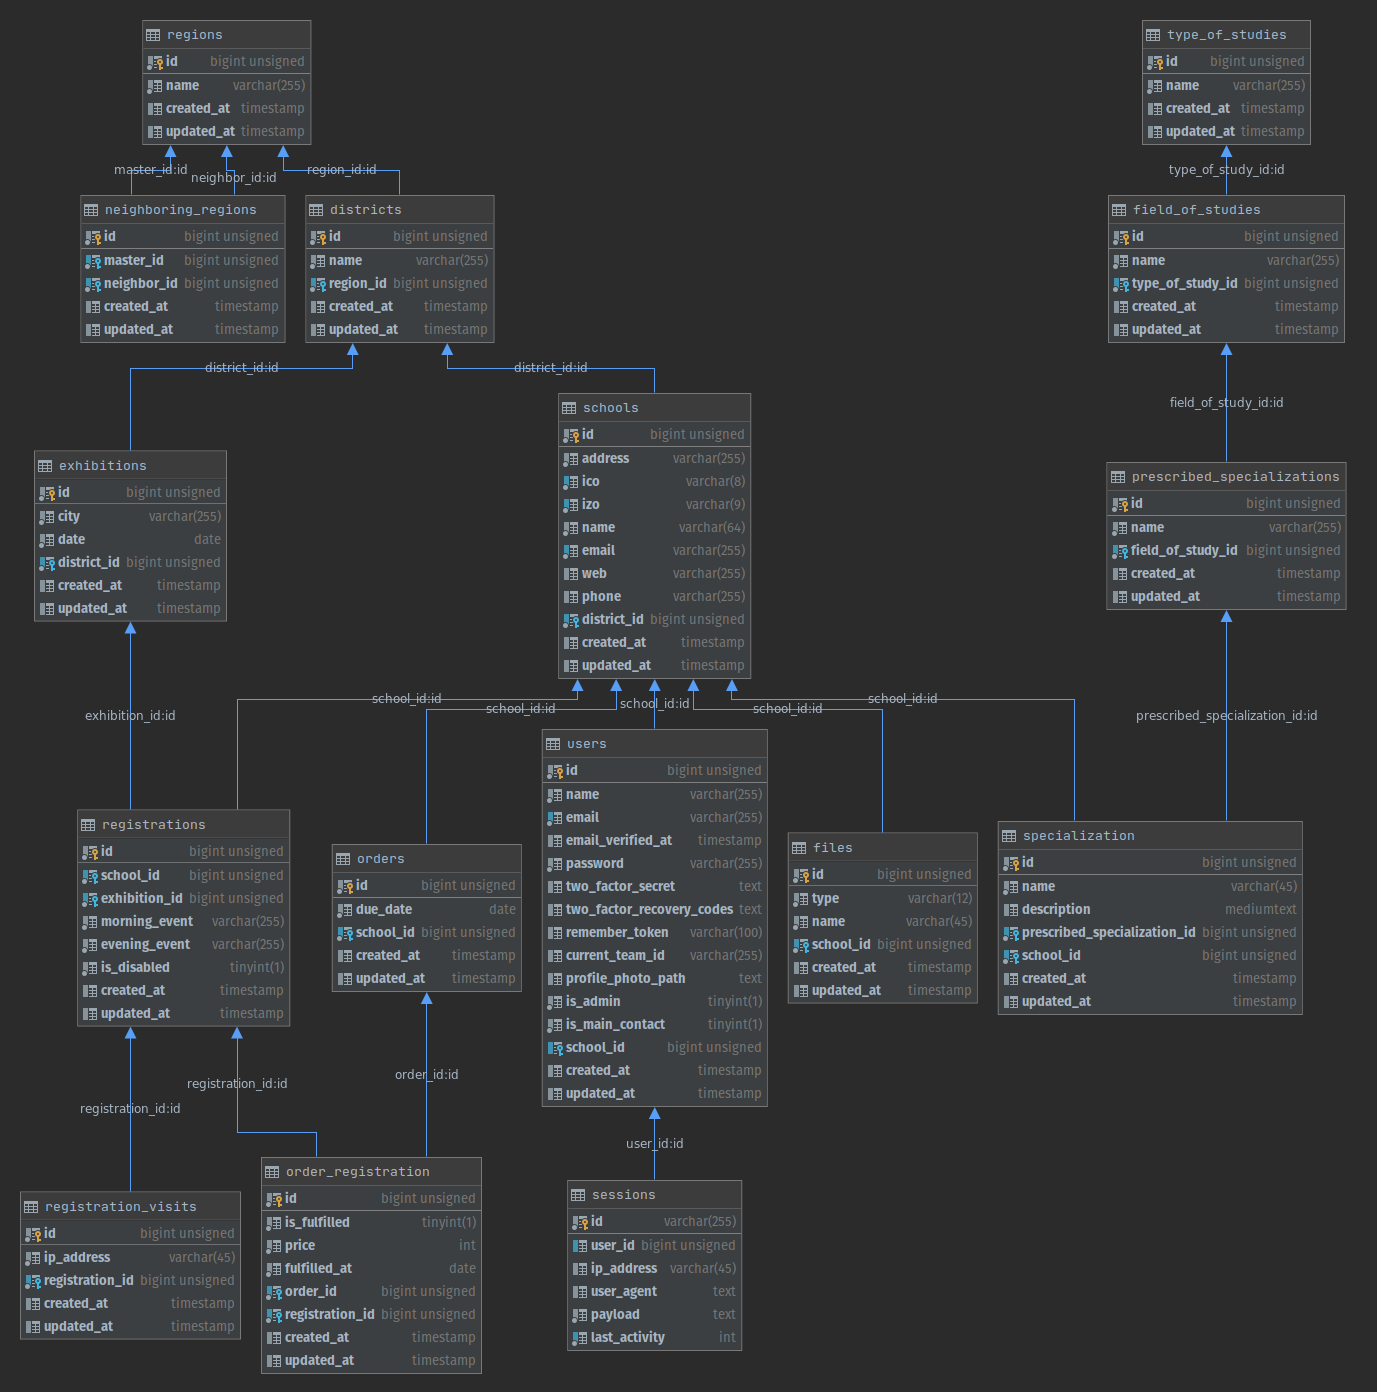
\includegraphics[width=\textwidth]{img/datovy-model-rijen-2020-2.png}
\caption{Datový model aplikace \bso  k říjnu roku 2020}
\label{fig:data-model-2020}
\end{figure}

Datový model \bso je postaven kolem konceptu vystavovatele, z implementačních důvodů reprezentováno tabulkou \emph{schools}. Vystavovatelé jsou hlavní cílová skupina portálu. Mají možnost přihlásit se na výstavy a vložit krátký článek o sobě, případně o svých oborech, s podporou formátování za pomoci \acrshort{html} značek. Portál umožňuje vystavovatelům nahrávat loga, informační brožury a obrázky, aby mohli zájemcům poskytnout maximální množství informací. V současné podobě projektu \bso existují tři typy vystavovatelů: školy, firmy a Úřady Práce České Republiky. 

Školy jsou hlavním typem vystavovatele. Mohou si vytvářet obory, které dále přiřazují k oborům z číselníku \acrshort{msmt}. To nám dovoluje poskytovat filtrování škol podle typu studia, zaměření a oborů samotných. Školy jsou také automaticky párovány s výsledky maturitních zkoušek, výsledku soutěží zařazených do programu Excelence \acrshort{msmt} a k inspekčním zprávám. Hlavní přínos portálu \bso pro školy je navázání kontaktu s žáky 9. tříd a propagace. 

Druhým významným typem vystavovatele jsou firmy. Ty mohou vyjádřit svou podporu školám skrze funkcionalitu spolupráce. Kromě toho mají možnost seznámit zájemce se svou nabídkou pracovních pozic a stipendijních programů. Úřady práce mohou poskytovat nerozhodným žákům rady a dopomoci jim k vybrání vysněného studijního oboru.
	
	\section{Vývoj projektu}

V~této sekci jsou popsány technologie využité při vývoji portálu \bso a důvody pro jejich výběr, postup vývoje projektu a získané zkušenosti.

\subsection{Využité technologie}
\label{sub:used-technologies}

Při vývoji projektu byl využit programovací jazyk \nameref{sub:php} s~\gls{framework}em  \nameref{subsub:laravel}. Pro \gls{real-time} funkcionality, jako chat a notifikace, byl využit \gls{open-source} implementace aplikace \nameref{subsub:pusher}, Laravel Websockets\cite{laravel-websockets}. Jako \acrshort{rdbms} jsem využil MySQL\cite{mysql}. Emailové služby pro aplikaci zajišťuje služba Amazon SES\cite{amazon-ses}.

\subsubsection{PHP a Laravel}

Jelikož byla na začátku projektu \bso klíčová rychlost dodání \gls{mvp} byl vybrán jazyk \nameref{sub:php} společně s~\gls{framework}em \nameref{subsub:laravel} z~důvodu jednoduchosti nasazení, nízkých nákladů na provoz a velké flexibility a rychlosti vývoje. Dalším velkým plus jsou pomocné utility jako Composer\cite{composer} nebo Laravel Artisan Console\cite{laravel-artisan} a rozšíření Laravel Idea\cite{laravel-idea} pro \acrshort{ide} PhpStorm\cite{phpstorm}.

Laravel, skrze Laravel Jetstream\cite{laravel-jetstream}, poskytuje předpřipravené části aplikace jako registrace a ověřování uživatelů, \acrshort{css} \gls{framework} Tailwind CSS\cite{tailwind-css} a JavaScriptový \gls{scaffolding} Inertia.js\cite{inertia-js} nebo Laravel Livewire\cite{laravel-livewire}.

\begin{figure}[h]
\centering
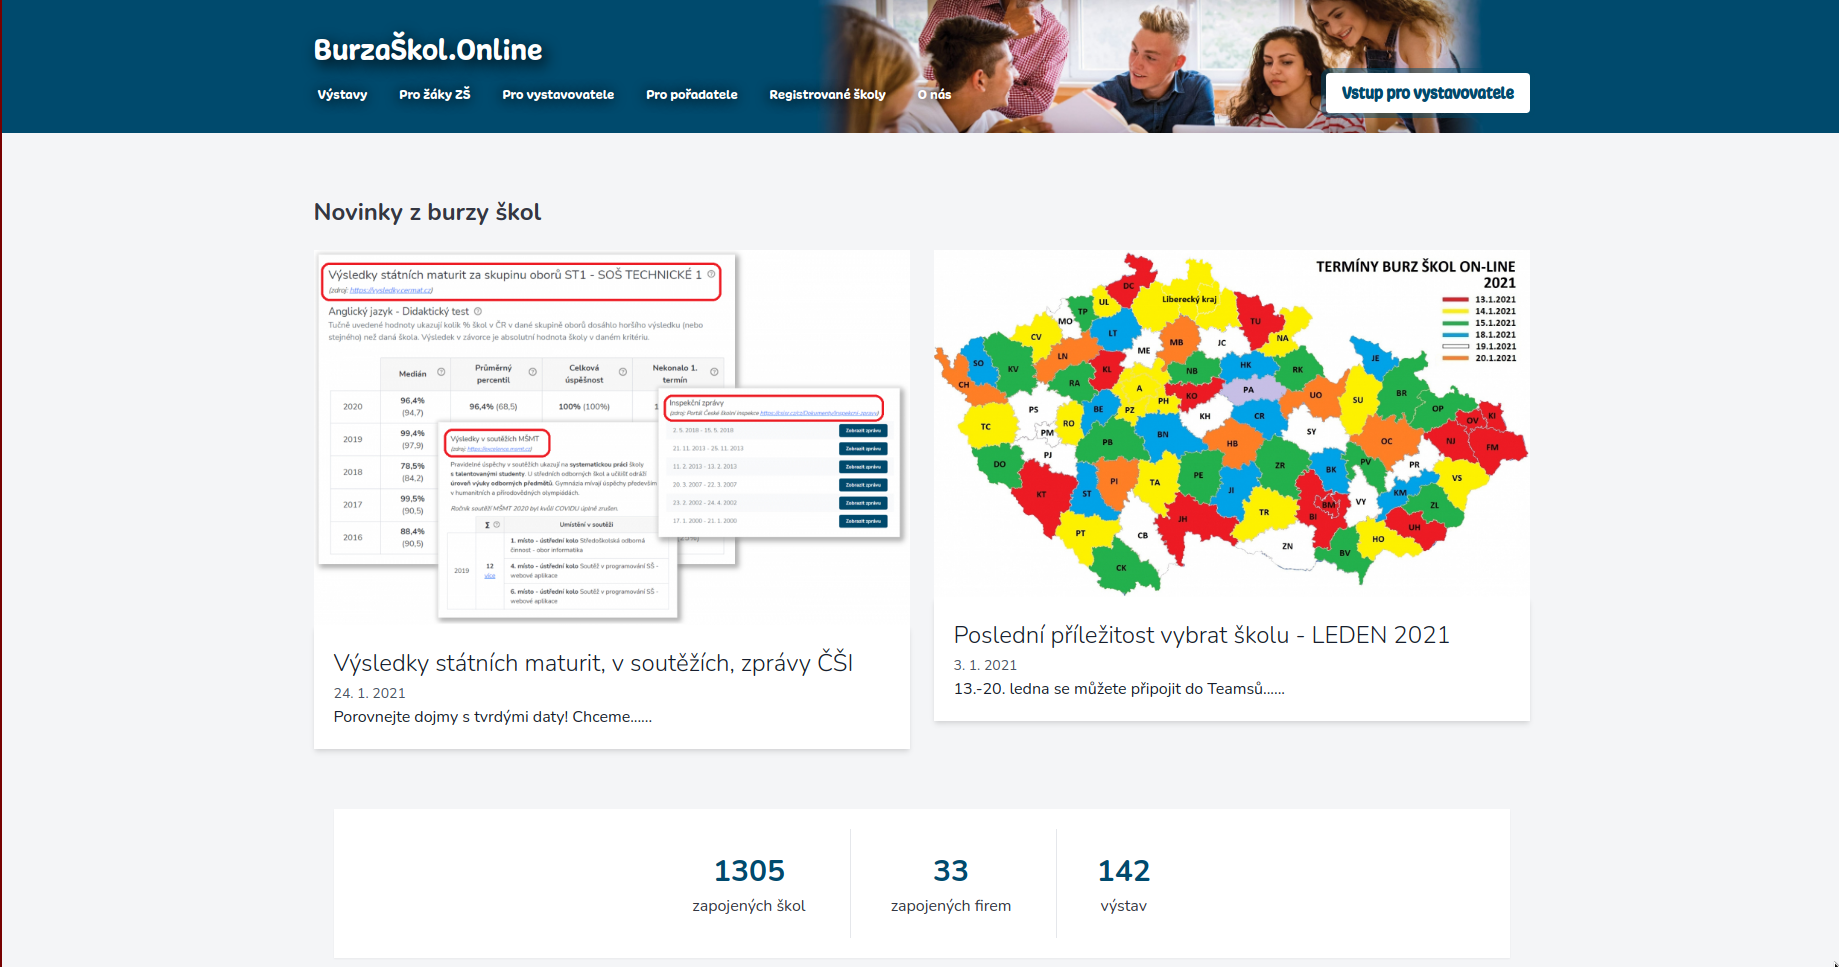
\includegraphics[width=\textwidth]{img/burzaskol-online.png}
\caption{Aplikace \bso}
\label{fig:burzaskol-online-2020}
\end{figure}

\subsubsection{Pusher}

Technologii Pusher byla vybrána z~důvodu jednoduché integrace do stávajícího projektu a možnosti pokročilého ladění. Z~implementačních důvodů byla využita \gls{open-source} implementace protokolu Pusher nazvaná \uv{Laravel Websockets}. To nám poskytlo větší kontrolu nad nasazením a škálováním projektu.

\subsubsection{MySQL}

\acrshort{rdbms} MySQL oproti ostatním relačním databázím vyniká jednoduchostí správy a množstvím poskytovatelů spravovaných databázových instancí\cite{mysql-vs-others}. To, a excelentní integrace s~jazykem \acrshort{php} a \gls{framework}em Laravel, z~ní dělá ideální volbu pro vývoj webových aplikací. Velkým přínosem je také široká řada nástrojů jako mysqldump\cite{mysqldump} nebo phpMyAdmin\cite{phpmyadmin}, které významně zjednodušují správu a provoz databáze MySQL.

\subsubsection{Amazon SES}

\acrfull{aws} poskytuje v~rámci služby \acrfull{aws-ses} jednoduchou a cenově dostupnou emailovou bránu. Ta nabízí funkcionality jako \gls{dkim} podepisování emailů a zobrazování pokročilých statistik jako počet odeslaných emailů, počet \uv{odražených} emailů\cite{email-bounce} a počet stížností na námi zaslanou poštu.

\subsection{Přípravy na vývoj projektu}

Předtím než může započít vývoj \acrshort{sw} projektu je zapotřebí se zadavatelem vytvořit zadání. Jedná se o~dokument popisující jednotlivé konkrétní funkcionality a procesy aplikace. Ze zadání by měly vycházet veškeré části aplikace jako je datový model a použité technologie. \emph{Zadání by mělo být konkrétní a jednoznačné, pokud existuje více výkladů, může dojít k~velkým problémům při vývoji aplikace.} 

Dalším krokem je výběr technologií, které budou na vývoj projektu použity. Ze zadání určíme pro jakou platformu bude projektu určen, zda-li se jedná o~webovou, desktopovou, mobilní nebo serverovou aplikaci. Dle toho vybereme konkrétní technologie jako např Laravel\cite{laravel} pro vývoj aplikace, MySQL\cite{mysql} pro ukládání dat a Git\cite{git} pro správu zdrojového kódu.

Když jsou zvoleny technologie můžeme začít vytvářet datový model pro vybraný typ databáze. Dále rozvrhneme jednotlivé obrazovky a postupy, které bude aplikace obsahovat. Je také potřeba vytvořit plán nasazení projektu, tedy jak bude aplikace hostováná, či jaký mail server využijeme.

Když máme všechny přípravy hotovy můžeme přejít k~samotnému programování projektu.

\subsection{Vývoj projektu ve frameworku Laravel}
\label{sub:laravel-development}

Prvním krokem při vývoji projektu \inlaravel, je vytvoření tříd tzv. \emph{modelů}\cite{laravel-models} a k~nim náležejících \emph{migrací}\cite{laravel-migrations}. Ty vytvoříme dle připraveného datového modelu.

Když jsou modely a migrace úspěšně vytvořeny můžeme přistoupit k~vytváření \emph{kontrolerů}\cite{laravel-controller}, \emph{komponent}\cite{laravel-blade-component} a definování \emph{cest}\cite{laravel-routes}.

\subsubsection{Modely}

Modely jsou \acrshort{php} třídy reprezentující samostatné databázové tabulky, řádky a relace mezi nimi. Modely nám dovolují vytvářet, upravovat a filtrovat záznamy jako by se jednalo o~nativní \acrshort{php} objekty. To velice zjednodušuje práci s~daty.

V~současné době aplikace \bso obsahuje 26 modelů, např. \emph{School} pro vystavovatele nebo \emph{Region} pro kraj. 

\subsubsection{Migrace}

Migrace, \inlaravel, slouží pro kontrolované úpravy databáze. Jejich hlavní úkol je udržet databázi v~konzistentním stavu s~verzí aplikace. Při nasazení nové verze tedy stačí spustit migrace a databáze je synchronizována s~verzí aplikace.

\subsubsection{HTTP cesty}

\acrshort{http} cesty definují jaký kód je spuštěn při \acrshort{http} požadavku. Cesta je identifikována pomocí jedné, či více \acrshort{http} metod a \acrshort{http} cesty. Cesta v~sobě může obsahovat parametry, např. id knihy. Cesta může vést na \emph{\acrshort{http} přesměrování}, \emph{\acrshort{php} funkci} nebo \emph{\acrshort{http} kontroler}.

Aplikace \bso definuje 38 unikátních \acrshort{http} cest. Velké množství \acrshort{http} cest dále přijmá různé parametry, které dále ovlivňují obsah vygenerované stránky.

\subsubsection{HTTP kontrolery}

\acrshort{http} kontrolery, \inlaravel, jsou \acrshort{php} třídy obsahující \expl{logiku pro zpracování \acrshort{http} cest}{handlery, \acrshort{php} metody}. Můžeme je rozdělit na standardní kontrolery, \emph{single-action kontrolery}\cite{laravel-controller-single-action} a \emph{resource kontrolery}\cite{laravel-controller-resource}.

Standardní kontrolery obsahují libovolný počet handlerů. Při definování \acrshort{http} cesty musíme definovat jak kontroler, tak metodu, která má být zavolána.

Single-action kontrolery obsahují pouze metodu \emph{\_\_invoke}. Jsou vhodné pokud je logika pro nějakou cestu velice komplexní a je lepší ji izolovat. Při definování cesty stačí zmínit pouze název třídy a \nameref{subsub:laravel} metodu automaticky spáruje.

Resource kontrolery mají přesně definovanou strukturu. Obsahují skupinu metod pro vytváření, úpravu a čtení daného \expl{zdroje}{resource}. Cesty se definují skupinově pomocí statické metody \emph{resource}.

\subsubsection{Blade komponenty}

Všechny aplikace mají za cíl zobrazovat uživateli informace. Webové aplikace využívají k~zobrazování informací značkovací jazyk \acrshort{html}.

U~jednoduchý stránek můžeme využít statických \acrshort{html} souborů, které jsou pro každý požadavek stejné a nemění se. Pro úpravu obsahu stránky je nutný přístup k~hostingové službě a znalost \acrshort{html}.

Moderní webové aplikace vyžadují obsah dynamický, který je závislý na velké řadě faktorů, např. zda-li je uživatel přihlášen, jaká jsou jeho oprávnění, či jaké výstavy se právě konají. Obsah těchto stránek je většinou uživatelsky editovatelný za pomocí grafického \acrshort{wysiwyg} editoru.

Pro generování těchto stránek se používají šablonovací nástroje jako samotné \acrshort{php} nebo různé pomocné knihovny jako Twig\cite{twig} nebo Laravel Blade Views\cite{laravel-blade}. Takové knihovny nám dovolují psát čisté \acrshort{html} s~přídavkem speciálních příkazů. Tyto příkazy nám dovolují například podmínečné generování, možnost vypisovat a formátovat \acrshort{php} proměnné nebo modularizaci stránek na menší znovupoužitelné komponenty.

	
	\section{Nasazení a provoz projektu}\label{sec:deployment-running}

Tato kapitola je věnována nasazení a provozu projektu \bso{}.
Popisuje volbu hostingové služby a serverovou architekturu.
Obsahuje také poznatky a překonané problémy, které v~průběhu nasazování projektu vznikli.

\subsection{Hostingová služba}
\label{sub:hosting}

Při navrhování projektu \bso{} byly zvažovány služby Amazon AWS\cite{amazon-aws}, Microsoft Azure\cite{ms-azure} a cloudem společnosti Digitalocean\cite{digitalocean}.
Všechny tři služby poskytují velké množství pokročilých funkcí pro vývoj a provoz webových aplikací. 

Nakonec byl pro většinu funkcí zvolen cloud společnosti Digitalocean, jelikož má ze všech tří poskytovatelů nejjednodušší správu a finanční politiku,
je přesně uvedeno za co platíte a neexistují žádné skryté limity a kvóty.
Mezi další výhody cloudu Digitalocean patří vysoký výkon a velmi příznivé ceny.\cite{digitalocean-advantages}

Pro další funkcionality jako ukládání souborů a zasílání emailů byly využity služby Amazon S3\cite{amazon-s3} a Amazon SES\cite{amazon-ses}.
Důvody pro toto rozhodnutí byly bezkonkurenční ceny a integrace s~použitými technologiemi, hlavně \gls{framework}em \nameref{subsub:laravel}.


\begin{figure}[!ht]
\centering
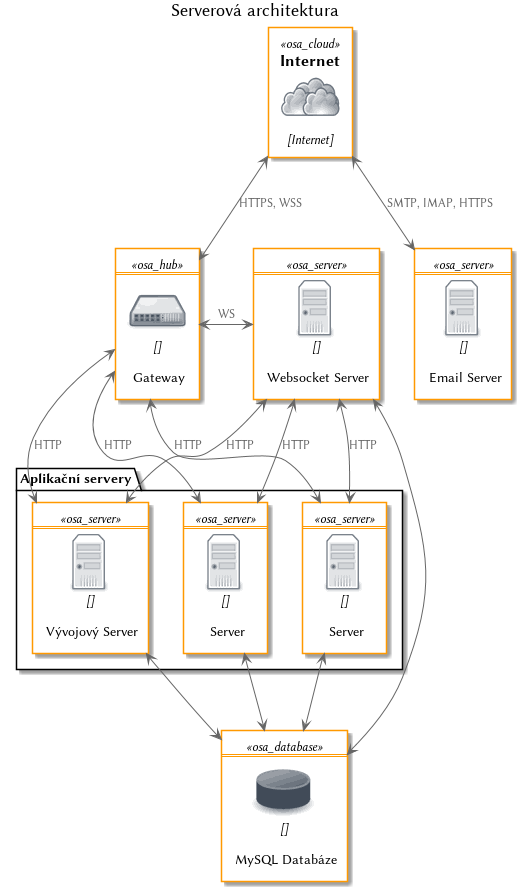
\includegraphics[width=11cm]{img/serverova-architektura.png}
\caption{Serverová architektura projektu \bso{}}
\label{fig:servery}
\end{figure}

\clearpage

\subsection{Serverová architektura}

\emptyLine

\begin{displayquote}
\textit{Internet je divokým a nebezpečným místem\cite{internet-is-dangerous-place}.}
\end{displayquote}

\begin{displayquote}
\textit{\acrlong{sw} a \acrlong{hw} je nespolehlivý, chyba není výjimka ale pravidlo\cite{failure-is-rule-not-exception}.}
\end{displayquote}

\emptyLine

Podle těchto dvou faktů musíme řídit svůj návrh serverové infrastruktury.  Musíme tedy vytvořit serverovou infrastrukturu, která je odolná, bezpečná a škálovatelná.

Z~hlediska bezpečnosti můžeme rozdělit servery projektu \bso{} na dvě skupiny: \textit{okrajové servery} a \textit{interní servery}.

Okrajové servery mají za úkol komunikaci s~Internetem.
Jedná se o~několik přesně definovaných míst, skrze něž prochází všechna komunikace určená mimo naši infrastrukturu.

Jednou z~hlavních výhod tohoto přístupu je možnost využívat uvnitř naší infrastruktury nešifrované protokoly jako \acrshort{http}
a provádět jejich zašifrování pouze na těchto dedikovaných okrajových serverech.
Tyto nešifrované protokoly jsou výkonnější a jednodušší než jejich šifrované varianty\cite{http-faster-https}.
Z~důvodu bezpečnosti je nelze použít pro Internetovou komunikaci.

Z~pohledu resilience, obrany proti výpadku, jsou nejdůležitějšími opatřeními replikace a \hyperref[sub:load-balancing]{load-balancing} klíčových částí. Využíváme proto \hyperref[sub:load-balancing]{load balancery} a \hyperref[subsub:managed-databases]{spravované databáze}, u~kterých neznamená výpadek jednoho stroje nedostupnost celé aplikace.


\subsection{Postup nasazení aplikace}
\label{sub:deployment}

Prvním krokem je provize serveru. Jelikož projekt \bso{} obsahuje pouze malý počet serverů, bylo možné všechny servery nakonfigurovat a vytvořit přímo z~ovládacího panelu Digitalocean.

Poté co jsou servery vytvořeny přejdeme ke konfiguraci samostatných serverových rolí. Každá serverová role vyžaduje separátní konfiguraci a specifický software, aby mohla svou funkci vykonávat.

Dalším krokem je vytvoření obrazů disků nakonfigurovaných serverů, abych mohl rychle a jednoduše vytvářet další servery těchto rolí. Pro každou serverovou roli byl vytvořen seznam parametrů, které je po vytvoření serveru z~obrazu disku nutné upravit. U~aplikačních serverů je například nutné upravit \acrshort{ip} adresu, na které má webový server naslouchat pro nová připojení. 

Posledním krokem je nastavení příslušných \acrshort{dns} záznamů a získání \acrshort{ssl} certifikátů.

\subsection{Nasazování aktualizací aplikace}
\label{sub:update-deployment}

První přístup nasazování aktualizací, který byl v projektu \bso{} využit, byl založený na Github Actions\cite{github-actions}.
Github Actions je \gls{ci-cd} mechanismus založený na spouštění kódu v~závislosti na událostech verzovacího systému Git\cite{git}. Využíván byl SSH for Github Actions\cite{ssh-for-github-actions}, pro automatické nasazování při commitu do dedikované větve.

Tento přístup má několik problémů. Hlavním problémem je fakt, že pro každý přidaný cílový server je zapotřebí vytvořit novou konfiguraci. Když vysazovací akce selže, je těžké najít příčinu, jelikož výpisy Github Actions jsou nepřehledné a zaměňují \acrshort{stdout} a \acrshort{stderr}. Posledním velkým problémem tohoto přístupu je, že pro spuštění vysazení je zapotřebí změna v~kódu aplikace.

Tyto problémy jsem vyřešil použitím Laravel Envoy\cite{laravel-envoy}. Laravel Envoy využívá konfigurační soubory v~jazyce \acrshort{php} pro provádění dávek akcí na skupině serverů zároveň. Pokud je zapotřebí přidat nový server, stačí přidat jeho \acrshort{ip} adresu do seznamu serverů a Laravel Envoy automaticky provede všechny potřebné akce. Další velkou výhodou je absence nutnosti ukládat \acrshort{ssh} klíče na serveru třetí strany. Pro zopakování vysazení stačí pouze znovu spustit Laravel Envoy.

	
	\section{Bezpečnost aplikace}
\label{sec:security}

Kapitola zaměřená na zabezpečení projektu \bso{} je z~důvodu komplexity tématu rozdělena na dvě části.  První část pojednává o~zabezpečení systému proti útokům vedeným skrze samotnou aplikaci, např. útokům typu \emph{\acrshort{sql} Injection}. Druhá kapitola se zaměří na zabezpečení infrastruktury proti útokům vedeným z~internetu cílících na špatně nakonfigurované služby, např. \emph{Útok na \acrshort{ssh} přihlašování serveru}.

\subsection{Aplikační zabezpečení}

Hlavní nebezpečí při provozování Webového portálu, plyne z~práce s~uživatelským vstupem. Aplikace musí tento vstup přijímat a operovat nad ním. To může vést k~celé řadě útoků. Je tedy důležité, aby uživatel svým vstupem nemohl webovou aplikaci napadnout, zpomalit, ani jinak vyřadit z~provozu. Nejdříve se zaměříme na bezpečnost textových polí a útoky s~nimi spojenými.

\subsubsection{SQL Injection}

\acrshort{sql} Injection\cite{sqlinject} je typ útoku, při kterém útočník zadá do textového vstupu kód v~jazyce \acrshort{sql}. Naše aplikace poté tento kód vezme a přímo ho vloží do řetězce dotazu.Při vykonávání příkazu pak databázový server vykoná tento škodlivý kód, jako by pocházel od samotné aplikace.

Tento útok představuje velké nebezpečí, jelikož může vést od ztráty dat, až k~úniku citlivých dat do rukou útočníka.

Aplikace \bso{} se proti tomuto typu útoku brání pomocí \emph{předpřipravených dotazů}\cite{mysqlprepstmt}. Jedná se o~techniku, kdy je databázový dotaz rozdělen na dvě části. První část tvoří samotné příkazy, které popisují, jak bude daný dotaz proveden. Druhou část tvoří uživatelské vstupy. Tato část obsahuje pouze data a databázový server ji nikdy nespouští. Tím zabraňuje tomu, aby server vykonal uživatelský vstup jako příkaz. \emph{Předpřipravené dotazy}\cite{mysqlprepstmt} riziko tohoto útoku plně eliminují.

\subsubsection{Cross-site skriptování}

Cross-site skriptování\cite{xss}, nebo také \acrshort{xss}, je typ útoku, při kterém je do textového vstupu zadán validní kód spustitelný prohlížečem. Zranitelný webserver poté tento kód vloží přímo do stránky, která je zaslána na klientské zařízení. Klientské zařízení tento škodlivý kód následně vykoná v~domnění, že se jedná o~kód naší aplikace.

Tento útok představuje pro návštěvníky velké nebezpečí, jelikož může vést ke krádeži uživatelských přihlášení, zobrazování reklam nebo krádeži platebních údajů.
Mezi stránkové skriptování\cite{xss} může být také využito jako mezikrok pro další, např. phishingové\cite{phishing}, útoky.

Potenciálními místy, kde by mohlo u~aplikace \bso{} k~napadení XSS dojít, jsou jednořádková vstupní pole a grafické textové editory. Jednořádková vstupní pole slouží pro jednoduchý uživatelský vstup bez formátování. Zabezpečení je tedy velice jednoduché. Jakýkoliv vstup, který uživatel zadá, je očištěn a veškeré \acrshort{html} značky jsou odstraněny. U~grafických textových editorů však není tato obrana možná, jelikož validním vstupem je i \acrshort{html} kód. Aplikace tedy daný kód na serveru parsuje a odstraní veškeré závadné \acrshort{html} značky, jako je například značka \emph{script}, a závadné \acrshort{html} atributy, jako například \emph{onmove}.

\subsubsection{Podvržení požadavků mezi stránkami}

Podvržení požadavků mezi stránkami (\acrshort{csrf}) \cite{csrf} je typ útoku, při kterém cizí stránka obsahuje odkaz, který vede na naši webovou adresu. Většinou se jedná o~požadavky typu POST\@. Tento požadavek má většinou za cíl vykonat škodlivou akci, např. napsat příspěvek bez vědomí uživatele. Při útoku je využíváno faktu, že prohlížeč s~každým požadavkem odesílá \acrshort{http} cookies, které ověřují uživatele serveru.

Útočník tedy může například vytvořit novou objednávku a tím způsobit finanční újmu. Tento útok představuje pro uživatele velké nebezpečí.

Aplikace \emph{BurzaŠkol.Online} se brání podvržení požadavků tak, že pro každou uživatelskou akci vyžaduje tzv. \acrshort{csrf} Token\cite{csrf}. Token je unikátní pro každý požadavek a dovoluje uživateli vykonat přesně jednu akci. Token je vygenerován serverem, přímo do \acrshort{html} kódu stránky. Útočník k~němu proto nemá přístup a není mu dovoleno vykonat žádnou akci.

\subsubsection{Útok hrubou silou}

Útoky hrubou silou\cite{bruteforce} je skupina útoků využívající velkého počtu požadavků za účelem uhodnutí uživatelských přihlašovacích údajů. Tyto požadavky jsou vedeny na přihlašovací formulář aplikace a podle odpovědi serveru určují zda byl útok úspěšný, či nikoliv.

Útok typu brute-force vede k~vyzrazení přihlašovacích údajů útočníkovi. Útočník tím získá možnost plné kontroly nad uživatelským účtem.

Proti tomuto útoku je nasazena obrana spočívající v~limitaci počtu požadavků na \acrshort{ip} adresu. Pokud uživatel udělá za určený časový více požadavků na přihlášení než je povolený limit, tak aplikace požadavky zahazuje a dále je nezpracovává. Tato ochrana činí útoky typu brute-force velice nepraktické, až nemožné.

\subsection{Zabezpečení infrastruktury}

Dalším důležitým faktorem bezpečnosti, při provozování webového portálu, je zabezpečení serverové infrastruktury. Útoky na serverovou infrastrukturu aplikace mají často větší dopad než zranitelnosti aplikace samotné. Tyto útoky mají často za úkol aplikaci vyřadit z~provozu nebo ji zneužít. Jedná se, např. o~\emph{slovníkové útoky nebo bruteforce útoky na \acrshort{ssh} přihlašování} nebo o~\emph{denial of service} útoky.

\subsubsection{Útoky na SSH přihlašování}

Při útoku na SSH přihlašování serveru se využívá povoleného přihlašování pomocí uživatelských hesel. Útok se snaží najít kombinace uživatelských jmen a hesel, které nejsou dostatečně komplexní a bezpečné. Častým cílem útoku je kořenový uživatel, \emph{root}, který by úspěšnému útočníkovi poskytl kompletní kontrolu nad cílovým strojem. K~prolomení hesel se využívají tzv.\ slovníkové útoky - soubory velkého množství častých hesel, kterými se útočník snaží zabezpečení prolomit.

Pokud dojde k~prolomení \acrshort{ssh} přihlášení serveru získá tím útočník plný přístup k~serverovému terminálu. Je tedy schopný vykonávat všechny akce, ke kterým má napadený účet oprávnění. Útočník může například zapojit stroj do botnetu\cite{botnet}, zfalšovat nebo zaměnit poskytované stránky, či ukrást platební nebo osobní údaje.

Jednou z~hlavních obran proti tomuto útoku je zákaz používaní hesel pro vzdálený přístup. K~přihlašování se poté využívá tzv. \acrshort{ssh} klíčů\cite{ssh-keys} - certifikátů založených na asymetrické kryptografii. Druhou linií obrany je poté rozřazení jednotlivých úloh pod samostatné uživatelské účty a princip minimálních oprávnění. Toto opatření pak minimalizuje škody způsobené útočníkem na úzkou napadenou oblast. 

\subsubsection{Denial of service útoky}

Útoky typu \acrfull{dos}\cite{denial-of-service} jsou útoky při kterých se útočník snaží zahltit naši infrastrukturu, a tím způsobit její výpadek.
Nejčastější variantou \acrshort{dos} útoku je \acrfull{ddos} - \acrshort{dos} útok vedený z~mnoha míst najednou \cite{distributed-denial-of-service}. 
Vyskytují se ve velkém množství variací, např. Slowloris, různé typy floodingu a amplifikační útoky.

\subsubsubsection{Slowloris útoky}

\noindent
\acrshort{dos} útok Slowloris\cite{slowloris} využívá toho, že každé připojení vyžaduje, tzv. \acrfull{fd}\cite{fd}. \acrshort{fd} je systémový zdroj, který v~unixových systémech reprezentuje otevřené soubory, či síťová připojení. Každý běžící proces má omezený počet \acrshort{fd}, které je schopný otevřít v~jednu chvíli. Cílem útoku Slowloris je donutit webserver k~vyčerpání počtu dostupných \acrshort{fd} tím, že otevře velkou spoustu připojení a zasílá pouze tolik dat, aby server připojení neuzavřel. Snaží se tak napodobit spoustu zařízení s~pomalým připojením. Když dojde k~vyčerpání volných \acrshort{fd} ztratí server schopnost přijímat nové požadavky a na koncového uživatele působí jako přetížený. Hlavní výhoda tohoto útoku je, že nevyžaduje větší prostředky ke svému provedení. Hlavní obranu proti útoku tvoří omezení maximálního množství připojení na \acrshort{ip} adresu. Je také nutné nastavit rozumnou spodní hranici rychlosti připojení.

\subsubsubsection{Floodingové útoky}
\label{subsec:ddos-flood-attack}

\noindent
Floodingové \acrshort{ddos} útoky jsou založené na přetížení cílového stroje. Jejich cílem je překročení maximální propustnosti \acrshort{hw} a \acrshort{sw} komponent serveru, a tím způsobit nedostupnost, výpadek, či dokonce fyzické poškození. Tento útok využívá nedokonalosti různých protokolů a jejich implementací. Příkladem floodingových útoků je UDP flood\cite{udp-flood}, SYN flood\cite{syn-flood} nebo HTTP flood\cite{http-flood}.

\subsubsubsection{Amplifikační útoky}

\noindent
Amplifikační \acrshort{ddos} útoky jsou variantou \hyperref[subsec:ddos-flood-attack]{floodingových útoků} využívající základní internetové služby, jejichž velikost odpovědi je několikanásobně větší než velikost požadavku. U~některých dotazů je poměr až 1:200 \cite{ddos-amplify-ratio}. Hlavními cíli amplifikačních útoků jsou nechráněné \acrshort{ntp} servery\cite{ddos-amplify-ratio} a \acrshort{dns} servery\cite{dns-flood}. Při útoku se využívá faktu, že některé \acrshort{ntp} a \acrshort{dns} servery přijímají požadavky pomocí \acrshort{udp} protokolu, bez kontroly pravosti zpáteční \acrshort{ip} adresy. Útočník zašle malý \acrshort{udp} požadavek s~podvrženou \acrshort{ip} adresou cílového serveru. Zranitelný server poté odpoví na podvrženou \acrshort{ip} adresu a provede \acrshort{udp} flood útok pod záminkou odpovědi na legitimní dotaz.

\subsubsubsection{Obrana proti floodingovým a amplifikačním útoků}

\noindent
Obrana proti floodingovým a amplifikačním útokům je velice náročná. Jeden z~největších problémů je fakt, že škodlivý datový provoz je v~mnohých případech těžce rozeznatelný od normálního datového provozu aplikace. Je proto potřeba izolovat útočící \acrshort{ip} adresy od \acrshort{ip} adres legitimních uživatelů. Problém s~blokací škodlivého provozu těchto útoků je, že samotný objem blokovaných dat má potenciál naši infrastrukturu přetížit. Ideálním, i když nákladným, řešením jsou fyzické firewally, které upravují provoz pomocí hardwarových akcelerátorů. Méně efektivními, ale stále užitečnými, možnostmi je alokace větších serverových prostředků na místa, kde naše služby komunikují s~veřejným internetem, v~kombinaci s~blokováním útočících \acrshort{ip} adres. 

	
	% TODO: vymyslet lepší nadpisy

\section{Postup projektu}

V této sekci je popsáno praktické nasazení projektu \bso{}.

\subsection{Jedno-serverové nasazení}

První verze aplikace \bso{} využívala pouze jeden server pro hostování všech aplikačních funkcí jako \acrshort{webserver}, databázový server a aplikační server. Tento způsob hostování má však mnoho problémů.

Jelikož celá infrastruktura běží na jednom serveru narážíme na velké bezpečnostní riziko vytvářením kritického bodu infrastruktury, jehož nedostupnost nebo porucha znamená výpadek celé aplikace. 
To také znamená, že není možné aplikaci aktualizovat bez jejího výpadku. 

Druhým, i když menším problémem, je omezení možnosti škálování v~odpovědi na nárůst požadavků, jelikož pro alokaci větších serverových prostředků je nutné server vypnout.
Pro aplikaci \bso{} toto nepředstavovalo velký problém jelikož jazyk \acrshort{php} je velice efektivní ve využívání serverových prostředků a provoz aplikace nepřekročil alokované serverové prostředky.

\subsection{Více-serverové nasazení}

Pro vyřešení tohoto problému byla \hyperref[fig:servery]{infrastruktura byla rozšířena} na více serverů. 

Jako vstupní bod infrastruktury byl vyčleněn server označen \textit{gateway}.
Mezi hlavní role tohoto serveru byly určeny \hyperref[sub:load-balancing]{load-balancer} a vstupní bod protokolů \acrshort{http} a \acrshort{ws}.
To nám dovoluje provádět provizi ssl certifikátů a ssl terminaci pouze v jednom místě naší infrastruktury.

Jelikož \textit{gateway} poskytuje služby \hyperref[sub:load-balancing]{load-balanceru} mohlo být vytvořeno několik, na sobě nezávyslých, instancí aplikace \bso{}.
Pro provedení tohoto kroku bylo zapotřebí rozčlenit všechny zdroje dat, např. \acrshort{rdbms} nebo ukládání souborů, na dedikované servery, jelikož aplikační servery nemohou tyto služby mezi sebou sdílet.
Jako \acrshort{rdbms} byla využita spravovaná databáze společnosti Digitalocean s replikací a automatickou správou redundantních serverů.
Na ukládání souborů bylo využito objektové úložiště Amazon S3 pro manipulaci se soubory ze všech aplikačních serverů najednou, bez potřeby vlastní infrastruktury.

Rozčlenění aplikačních serverů nám poskytuje větší odolnost proti výpadku samostatných serverů, výpadek serveru neznamená výpadek aplikace, pouze zhoršení dostupnosti.
Také nám dovoluje aplikaci škálovat bez potřeby její odstávky.

\subsection{Problém s pracovními vlákny load-balanceru Nginx}

Při prvním veřejné výstavě uspořádané skrze platformu \bso{} docházelo při požadavcích na server k výpadkům a překročení časového limitu požadavku.
Po konzultaci souboru \verb|/var/log/nginx/access.log| bylo zjištěno, že na serveru \textit{gateway} došlo k vyčerpání \acrshort{fd}.
To vedlo k nemožnosti spracování požadavků serverem.

Pokud není webový server schopný odpovědět v časovém limitu zobrazí webový prohlížeč stránku jako nedostupnou,
jelikož webové prohlížeče implementují časový limit pro požadavky\cite{browser-timeout}.

Pro opravu této chyby bylo zapotřebí zvýšit počet požadavků spracovávaných jedním pracovním vláknem a horní limit \acrshort{fd}.
Tyto změny byly provedeny v souboru \verb|/etc/nginx/nginx.conf|.
Zvýšení počtu požadavků, které je schopné jedno pracovní vlákno spracovat bylo zvýšeno použitím direktivy.
\begin{verbatim}
events {
      worker_connections <počet připojení>;
}
\end{verbatim}
Pro zvýšení horního limitu \acrshort{fd} byla použita direktiva \verb|worker_rlimit_nofile <počet FD>|.

\section{Provoz a přínos aplikace}


Ve špičce provozu aplikace \bso{} využíval \hyperref[sub:load-balancing]{load-balancer} asi 30\si{Mb/S} síťového provozu.
Systém v~tu dobu navštívilo asi 790 návštěvníků, tj.\ kolem 25 návštěvníků na školu\footnote{Čísla nejsou exaktní z~důvodu nemožnosti přesného měření návštěvnosti webových stránek.}.

\subsection{Zapojení škol}

Během prvních 14-ti dní projektu se v Pardubickém Kraji, díky podpoře odboru školství, zapojilo více jak 60\% středních škol.
V ostatních krajích bylo, i přes podporu \acrshort{msmt}, zapojení škol pouze sporadické.
Pokrok ale nastal po zapojení Úřadu práce na celostátní úrovni, kdy jediný dopis informačním a poradenským střdiskům přinesl zapojení více než 250 škol z celé České Republiky.
Zapojení úřadu práce nám také poskytlo další komunikační kanál se základními školami.

\begin{figure}[h]
\centering
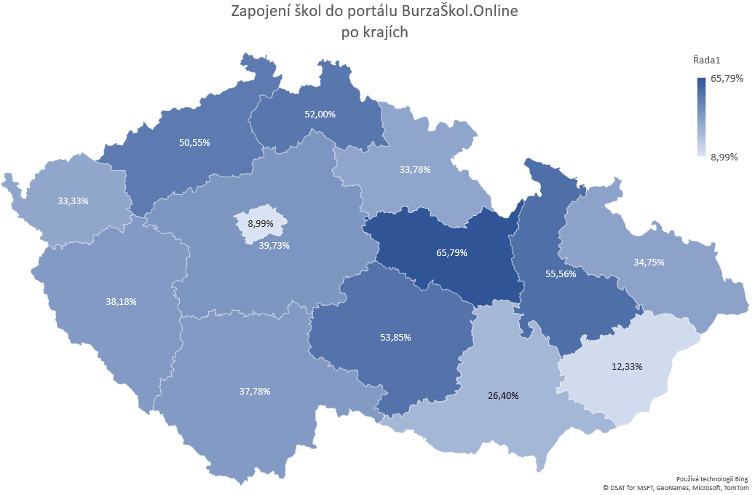
\includegraphics[width=\textwidth]{img/kraje-zapojeni.png}
\caption{Zapojení škol v jednotlivých krajích}
\label{fig:kraje-zapojeni}
\end{figure}

% tohle musí přesvědčit porotu o  tom, že si s nasazením nevymýšlíte.
% které bude na kolika serverech se to replikuje, jak vytížené jsou, jak vytížený je load-balancer,

\section{Přínos aplikace}

% tohle musí přesvědčit porotu o společenském přínosu, smysluplnosti aplikace 

% kolik v systému bylo škol, kdy byl nasazen poprvé a kolik se přes něj uskutečnilo spojení.

	
	\chapter*{Závěr}
\addcontentsline{toc}{chapter}{Závěr} % přidá položku závěr do obsahu

V~rámci práce byl vytvořen webový portál, který umožňuje nahrazení prezenčních Burz škol on-line 
videokonferencemi v~době pandemie koronaviru Covid-19.
Webový portál byl vyvinut a nasazen na takových technologiích a s takovou architekturou, 
abychom mohli pružně reagovat na výrazné kolísání požadavků na výkon odpovídající termínům on-line burz.

Serverová infrastrukturu pro provoz portálu byla navržena a zvolena s ohledem na bezpečnost, stabilitu 
a předpokládanou návštěvnost. 

Veškeré překážky zjištěné při provozu projektu \bso{} byly úspěšně odstraněny a všechny stanovené cíle 
projektu byly úspěšně splněny.

V rámci verze portálu 2.0 byl navázán kontakt s~portálem AtlasŠkolství.cz z důvodu poskytování lepších 
služeb a dosažení většího počtu uživatelů. 
Veškerá funkcionalita portálu \bso{} je nyní postupně 
zapracovávána do portálu AtlasŠkolství.cz.

%V~rámci práce byl vytvořen webový portál, který umožňuje nahrazení prezenčních Burz škol on-line video konferencemi v~době pandemie koronaviru Covid-19.
%Pro vytvoření portálu bylo zapotřebí získat a zpracovat zadání projektu. 
%Vyvinout webový portál na takových technologiích a s takovou architekturou, abychom mohli pružně reagovat na výrazné kolísání požadavků 
%na výkon, odpovídající termínům on-line burz.
%Vytvořit serverouvou infrastrukturu pro provoz portálu s ohledem na bezpečnost, stabilitu a předpokládanou návštěvnost.
%\expl{Překážka zjištěna při provozu projektu \bso{}}{nedostatečná konfigurace load-balanceru Nginx} byla úspěšně odstraněna, viz. \nameref{sub:poor-nginx}.
%Všechny stanovené cíle projektu byly úspěšně splněny.
%
%V rámci verze portálu 2.0 byl navázán kontakt s AtlasemŠkolství.cz z důvodu poskytování lepších služeb a dosažení většího počtu uživatelů.
%Veškerá funkcionalita portálu \bso{} se postupně zapracovává do portálu AtlasŠkolství.cz.
\pagebreak

	
	\listoffigures
	\addcontentsline{toc}{chapter}{Seznam obrázků}
	
%	\section*{Literatura}
	\printbibliography[title=Literatura]
	\addcontentsline{toc}{chapter}{Seznam literatury}
	
	
	%\listoftables
	%\addcontentsline{toc}{section}{Seznam tabulek}
	
	%\listoflistedequation
	%\addcontentsline{toc}{section}{Seznam rovnic}
	
	\printglossaries
	\addcontentsline{toc}{chapter}{Slovník}
\end{document}
